\documentclass[12pt,a4paper]{article}
\usepackage[T1]{fontenc}
\usepackage[brazil]{babel}
\usepackage[utf8]{inputenc}


\usepackage{ae,aecompl}
\usepackage{pslatex}
\usepackage{epsfig}
\usepackage{geometry}
\usepackage{url}
\usepackage{textcomp}
\usepackage{ae}
\usepackage{subfig}
\usepackage{indentfirst}
\usepackage{textcomp}
\usepackage{color}
\usepackage{setspace}
\usepackage{verbatim}



%Definindo as margens para 2cm e o espaçamento entre linhas para 1.5
% Relatório parcial deve ter espaçamento simples
%\linespread{1.5}

\geometry{ 
	a4paper,	% Formato do papel
	tmargin=25mm,	% Margem superior
	bmargin=25mm,	% Margem inferior
	lmargin=20mm,	% Margem esquerda
	rmargin=20mm,	% Margem direita
	footskip=20mm	% Espaço entre o rodapé e o fim do texto
}
\include{abaco} 
\renewcommand{\thetable}{\Roman{table}}
\newcommand{\x} {$\bullet$}


\begin{document}

% CAPA
\begin{titlepage}
\thispagestyle{empty}
  \begin{center} {\large \textbf{UNIVERSIDADE~ESTADUAL~DE~CAMPINAS}} \end{center}
  \begin{center} {\large INSTITUTO~DE~COMPUTAÇÃO}                    \end{center}
  \vspace{0.1cm}
  \begin{center}
  \begin{minipage}[tl]{31mm}
    \ABACO{1}{9}{6}{9}{1}
  \end{minipage}
  \end{center}
  \vspace{0.3cm}
  \begin{center} 
    {\large \textsc{Estudo da cache através de simulações
               }} 
    \\\vspace{0.5cm}
    {\textsl{Relatório do primeiro laboratório de MC723}}
    \\\vspace{1cm}
    \begin{tabular}{rl}
	  \textbf{Aluno}:       & Tiago~Chedraoui~Silva \\
	\end{tabular}
  \end{center}
  \vspace{0.5cm}

  \begin{abstract}
O princípio de funcionamento da memória cache é duplicar parte dos dados contidos na memória
principal (a memória lenta, neste caso) em um módulo menor (o cache) composto por dispositivos
de memória mais rápidos.
Quando o processador solicita um item de dado (gerando uma referência para seu endereço, que
pode ser físico ou virtual), o gerenciador de memória requisita este item do cache. Duas situações
podem ocorrer:
cache hit: item está presente no cache, é retornado para o processador praticamente sem período de
latência;
cache miss: item não está presente no cache, processador deve aguardar item ser buscado da memó-
ria principal.
Nesse laboratório, estudaremos a melhor organização de uma memória
cache para a execução de um determinado programa.

  \end{abstract}

  % Sumário
  \tableofcontents
\end{titlepage} 


% Guia para o relatório
%Quais são os principais parâmetros a serem definidos em uma cache?
%Quais são os valores típicos para esses parâmetros?
%Quais devem ser os limites mínimos e máximos desses valores?
%Olhe no manual do dinero e descubra quais desses parâmetros ele
%permite configurar -- Done
%Como podemos dizer que uma determinada configuração de cache é melhor que outra?
%O que é um trace de execução? -- Done +-
%Por que utilizar um trace de execução para achar a melhor configuração de cache para um programa?
%Por que escolher a melhor configuração de cache para um dado programa? A configuração de cache não é específica do processador?
%Olhe aqui qual o programa e número de arquivos você deve usar

%-----------------------------------------------------------------------------%
\section{Dinero}
%-----------------------------------------------------------------------------%

%Olhe no manual do dinero e descubra quais desses parâmetros ele permite configurar

O Software Dinero é um silmulador de cache para traces de memória
(registro de execução de um programa).

Dentre as opções de configuração da memória cache, o dinero nos
fornece as seguintes possibilidades:
tamanho da memória chace, tamanho do bloco da memória
cache, tamanho do sub-bloco, associatividade, política de
substituição (LRU\footnote{Least recently used: substitui a página na memória cuja última referência é a mais antiga.
}, FIFO\footnote{First-in, first-out: substitui a página mais antiga na memória} ou aletório), política de escrita se occorer um hit (write-back\footnote{Quando um ciclo de escrita ocorre para uma palavra, ela é atualizada
apenas no cache.}, write-through\footnote{Quando um ciclo de escrita ocorre para uma palavra, ela é escrita
no cache e na memória principal simultaneamente.}), política de escrita se occorer um
miss ( write-allocate\footnote{Com
  alocação em escrita:Se ocorrer um miss é alocado na cache
  uma linha para o dado escrito. Usando, na mairoria das vezes, com a política write-back}, no-write-allocate\footnote{Sem
  alocação em escrita:Se ocorrer um miss de
  escrita, uma linha não é alocada na cache para o dado escrito. Usado, na maioria das vezes, com a política write-through.}, fetch on write\footnote{No caso de um miss para escrita, item é trazido
  para o cache após atualizado, se foi alocado espaço para ele na cache.}, no fetch on write\footnote{No caso de um miss para a  escrita, item é
  atualizado apenas na memória principal, não sendo trazido para o cache.}).

Utilizamos dois tipos de traces, o F2B, que executa 2 bilhões de
instruções e o M2B que executa 2 bilhões de instruções depois de pular
50 bilhões. Logo os traces F2B tendem a ser mais rapidamente
executados e com um miss rate diferente do M2B, já que ambos
acessam posições diferentes da memória durante a execução das instruções. 

% -lN-Tsize P       Size
% -lN-Tbsize P      Block size
% -lN-Tsbsize P     Sub-block size (default same as block size)
% -lN-Tassoc U      Associativity (default 1)
% -lN-Trepl C       Replacement policy
%                   (l=LRU, f=FIFO, r=random) (default l)
% -lN-Tfetch C      Fetch policy
%                   (d=demand, a=always, m=miss, t=tagged,
%                    l=load forward, s=subblock) (default d)
% -lN-Twalloc C     Write allocate policy
%                   (a=always, n=never, f=nofetch) (default a)
% -lN-Twback C      Write back policy
%                   (a=always, n=never, f=nofetch) (default a)

%-----------------------------------------------------------------------------%
\section{Simulação}
%-----------------------------------------------------------------------------%

\subsection{Tamanho do bloco, associatividade, tamanho da cache}
\label{sec1}
O tamanho total de uma cache pode ser calculado pela multiplicação do
número de linhas, número de blocos por linha e tamanho dos blocos.
Uma cache L1 possui geralmente um tamanho entre 16KB e 128KB, podendo chegar, em algumas caches, a 8MB.

Para um determinado tamanho de cache e blocos, alterou-se a sua
associatividade. No qual percebe-se que o totalmente associado é o que
apresentou a melhor performance.

Posteriormente, aumentou-se o tamanho da memória cache total, deixando-a totalmente associada.
Percebeu-se que quanto maior a memória cache, menor é a taxa de miss. Contudo, vale ressaltar que
em certos momentos há uma estabilidade, ou seja, por mais que a cache cresça, a taxa de miss fica quase
constante.

Já o tamanho do bloco é relativo. De acordo com a figura \ref{tamBloco}, para cada valor de associatividade, um tamanho de bloco maior que 32
tende a ser melhor, porém após passar determinado valor ele tende a aumentar o valor de miss rate.

%\begin{figure}[H]
%\begin{centering}
%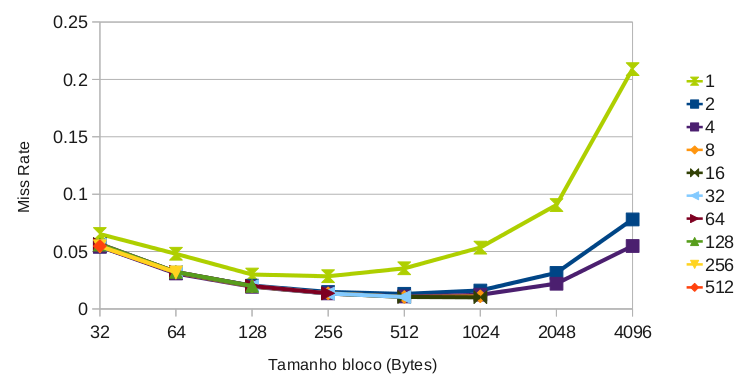
\includegraphics[scale=0.50]{graficos/grafico2}
%\par\end{centering}
%\caption{Alteração de associativade para vários tamanhos de bloco}
%\end{figure}

%\subsection{Uma Cache:  dados/instrução }


\subsection{Políticas de substituição}
Simulou-se a utilização das três políticas de substituição fornecida
pelo Dinero (Random, LRU e FIFO).
De acordo com a figura \ref{difPol}, para uma mesma configuração a política LRU foi a que apresentou um
melhor resultado.

%\begin{figure}[h!]
%\begin{centering}
%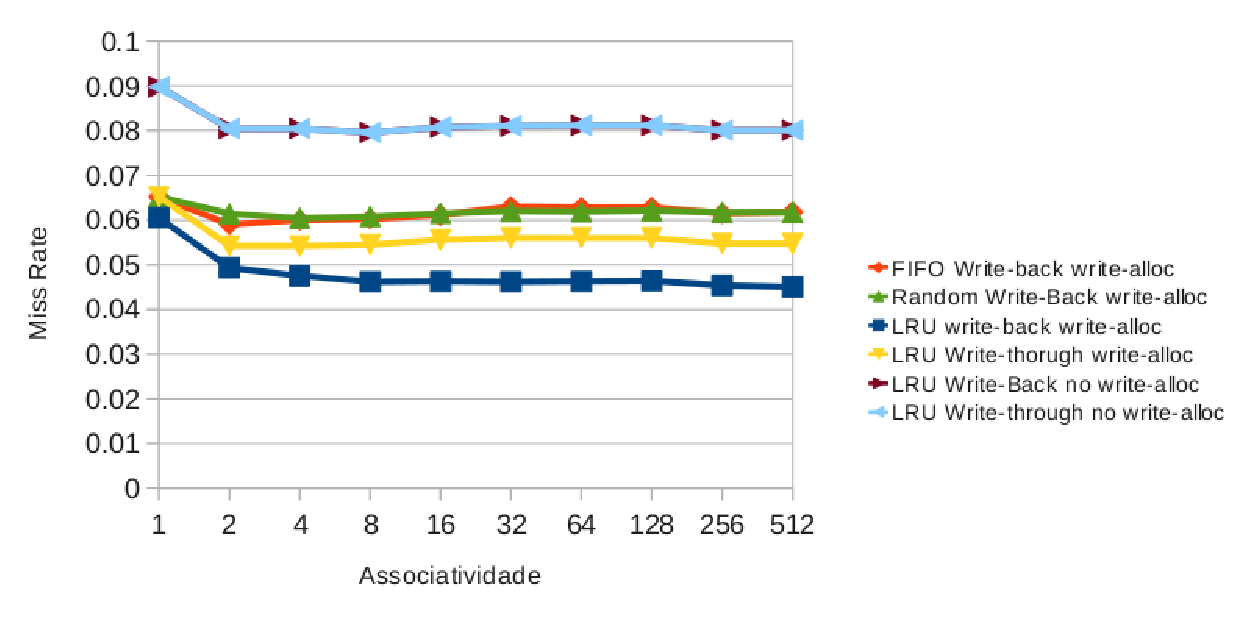
\includegraphics[scale=0.50]{graficos/grafico1}
%\par\end{centering}
%\caption{Diferentes políticas X Associatividade}
%\end{figure}


\subsection{Políticas de escrita se ocorrer um hit}
Simulou-se a utilização das duas políticas de escrita se ocorrer um
hit fornecida pelo Dinero.
De acordo com a figura \ref{difPol}, para uma mesma configuração a política write-back foi a que apresentou um
melhor resultado.

\subsection{Políticas de escrita se ocorrer um miss}
Simulou-se a utilização das duas políticas de escrita se ocorrer um
miss fornecida pelo Dinero.
Para uma mesma configuração, a política padrão, sempre usar Write allocate policy foi a que apresentou um
melhor resultado.

\begin{figure}[h!]
\subfloat[Alteração de associatividade para diferentes políticas]{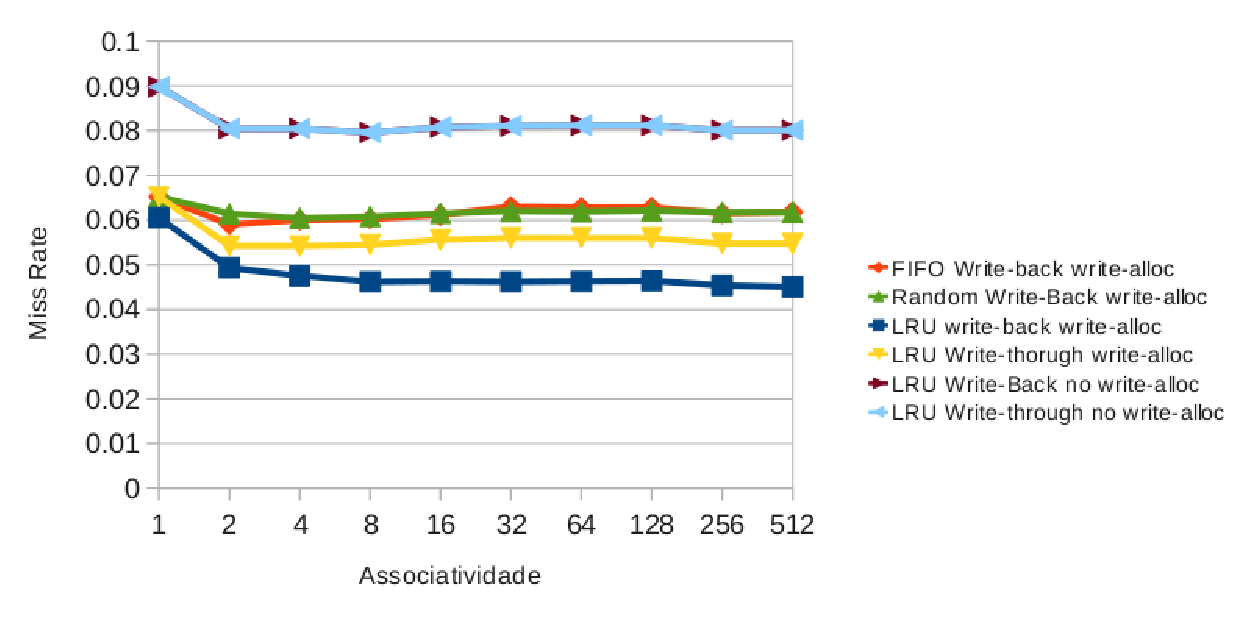
\includegraphics[scale=0.50]{graficos/grafico1}\label{difPol}}
\subfloat[Alteração de associativade para vários tamanhos de bloco]{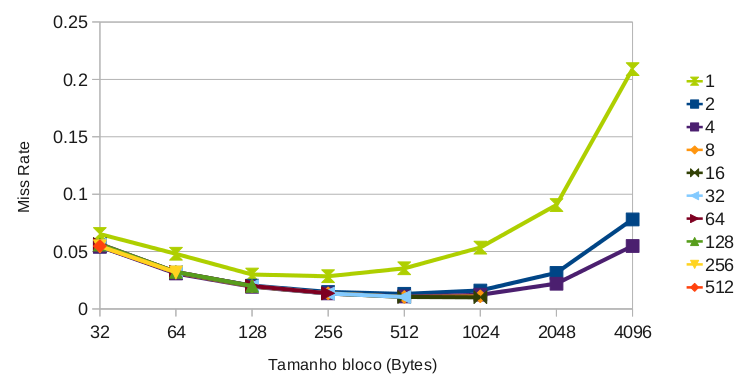
\includegraphics[scale=0.45]{graficos/grafico2}\label{tamBloco}}
\caption{Caches unificadas de 16KB com diversas configurações}
\end{figure}



\subsection{Duas caches:  dados e  instrução}
A memória cache pode ser separada em cache de instruções e para cache de dados,
de forma que dados e instruções poderiam ser acessados em paralelo. 
Vale ressaltar que o valor da taxa de miss será maior nas caches
separadas, contudo o tempo de acesso é menor.
Portanto, em uma comparação entre caches separadas e unificada, o tempo deve o fator de
escolha e não o miss rate. 
No entanto, para determinar-se a melhor configuração da cache, o miss
rate é essencial.


\begin{figure}[h!]
\subfloat[Cache de dados]{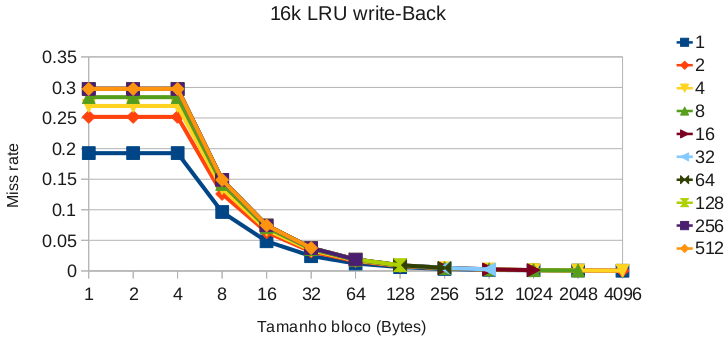
\includegraphics[scale=0.45]{graficos/grafico3}\label{cacheDados}}
\subfloat[Cache de instrução]{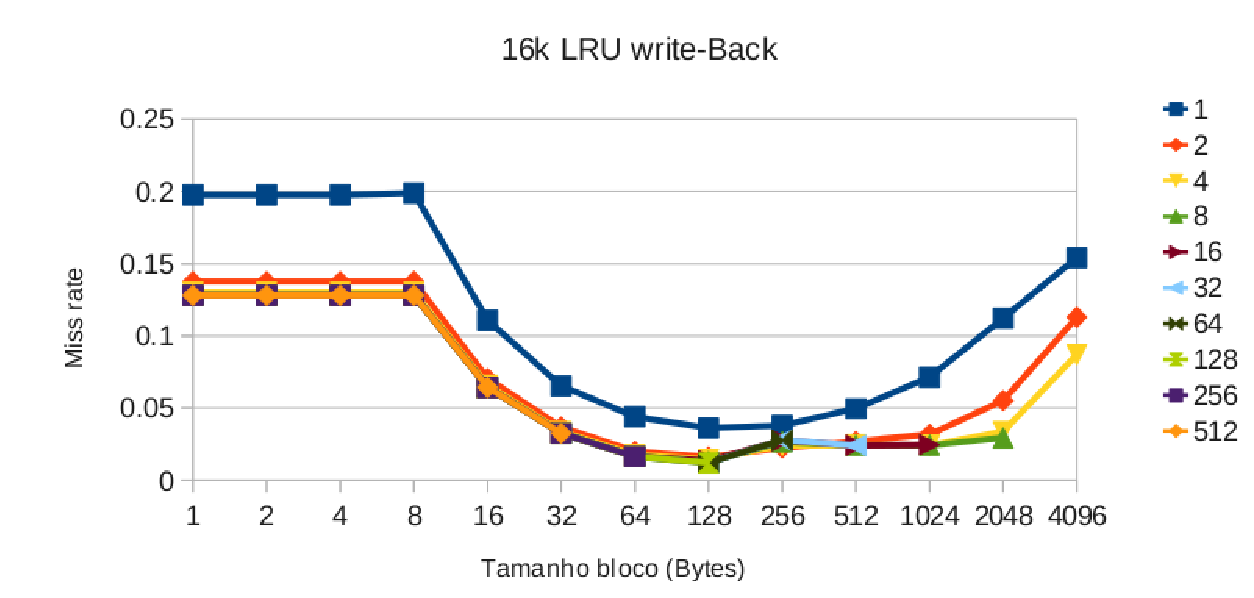
\includegraphics[scale=0.45]{graficos/grafico4}\label{cacheIns}}
\caption{Caches separadas:  Alteração de associativade para vários tamanhos de bloco}
\end{figure}

\section{Conclusão}
De acordo com nossas simulações, se considerarmos como fator de
escolha a taxa de miss rate e o custo de uma memória
cache\footnote{Queremos otimizar uma cache pequena em vez de possuir
  uma muito grande, o que teria uma eficiência melhor de acordo com a
seção \ref{sec1}}, escolheremos uma chace de 16KB, tamanho
de bloco 1024B, associatividade 16, política de substituição LRU.
o que nos proporcionou um valor de miss rate próximo a 1,01\% para o
trace m2b e 0.84\% para o trace f2b.

Por outro lado, se quisermos um tempo de acesso menor, dividiremos nossa cache
em uma de dados e outra de instrução.

De acordo com nossas simulações, se considerarmos a taxa de miss rate e o custo de uma memória
cache\footnote{Queremos otimizar uma cache pequena em vez de possuir
  uma muito grande, o que teria uma eficiência melhor de acordo com a
seção \ref{sec1}}, escolheremos uma cache de instrução de 16KB, tamanho
de bloco 4096B, associatividade 4 ou 2\footnote{Ambos valores de
  associatividade apresentaram mesma taxa de miss rate}, política de substituição LRU.
o que nos proporcionou um valor de miss rate próximo a 0.02\% para o
trace m2b e 0.04\% para o trace f2b.
E  escolheremos uma cache de dados de 16KB, tamanho
de bloco 128B, associatividade 128, política de substituição LRU.
o que nos proporcionou um valor de miss rate próximo a 4.48\% para o
trace m2b e 1.22\% para o trace f2b.

Se consideramos só possuirmos espaço para um total de 16KB de cache, 
escolheremos uma cache de instrução de 8KB, tamanho
de bloco 4096B, associatividade  2, política de substituição LRU.
o que nos proporcionou um valor de miss rate próximo a 0.03\% para o
trace m2b e 0.05\% para o trace f2b e uma cache de dados de 8KB, tamanho
de bloco 512B, associatividade 8, política de substituição LRU.
o que nos proporcionou um valor de miss rate próximo a 3.85\% para o
trace m2b e 3.12\% para o trace f2b.



% ******************************************************
% 		REFERENCIAS BIBLIOGRÁFICAS
% ******************************************************
%\section{Referências}
\bibliographystyle{plain}
\begin{small}
  \bibliography{referencias}
\end{small}

\end{document}
